% questions.tex —— 2008 年·普通高等学校招生考试·湖北卷·理科 · 题目内容片段（无答案）
% 由 tools/generate_projects.py 依来源总账自 2008/2008_数学真题_湖北理_试题.md 生成，勿手改（改源 MD 后重跑）


\gkpart{一、选择题}

\begin{question}
\gkti{1}设 $\boldsymbol a=(1,-2)$，$\boldsymbol b=(-3,4)$，$\boldsymbol c=(3,2)$，则 $(\boldsymbol a+2\boldsymbol b)\cdot\boldsymbol c=$（　）

（A）$(-15,12)$

（B）$0$

（C）$-3$

（D）$-11$

\end{question}
\begin{question}
\gkti{2}若非空集合 $A$，$B$，$C$ 满足 $A\cup B=C$，且 $B$ 不是 $A$ 的子集，则（　）

（A）“$x\in C$”是“$x\in A$”的充分条件但不是必要条件

（B）“$x\in C$”是“$x\in A$”的必要条件但不是充分条件

（C）“$x\in C$”是“$x\in A$”的充要条件

（D）“$x\in C$”既不是“$x\in A$”的充分条件也不是“$x\in A$”必要条件

\end{question}
\begin{question}
\gkti{3}用与球心距离为 $1$ 的平面去截球，所得的截面面积为 $\pi$，则球的体积为（　）

（A）$\dfrac{8\pi}3$

（B）$\dfrac{8\sqrt2\pi}3$

（C）$8\sqrt2\pi$

（D）$\dfrac{32\pi}3$

\end{question}
\begin{question}
\gkti{4}函数 $f(x)=\dfrac1x\ln\left(\sqrt{x^2-3x+2}+\sqrt{-x^2-3x+4}\right)$ 的定义域为（　）

（A）$(-\infty,-4]\cup[2,+\infty)$

（B）$(-4,0)\cup(0,1)$

（C）$[-4,0)\cup(0,1]$

（D）$[-4,0)\cup(0,1)$

\end{question}
\begin{question}
\gkti{5}将函数 $y=3\sin(x-\theta)$ 的图象 $F$ 按向量 $\left(\dfrac{\pi}3,3\right)$ 平移得到图象 $F'$，若 $F'$ 的一条对称轴是直线 $x=\dfrac{\pi}4$，则 $\theta$ 的一个可能取值是（　）

（A）$\dfrac5{12}\pi$

（B）$-\dfrac5{12}\pi$

（C）$\dfrac{11}{12}\pi$

（D）$-\dfrac{11}{12}\pi$

\end{question}
\begin{question}
\gkti{6}将 $5$ 名志愿者分配到 $3$ 个不同的奥运场馆参加接待工作，每个场馆至少分配一名志愿者的方案种数为（　）

（A）$540$

（B）$300$

（C）$180$

（D）$150$

\end{question}
\begin{question}
\gkti{7}若 $f(x)=-\dfrac12x^2+b\ln(x+2)$ 在 $(-1,+\infty)$ 上是减函数，则 $b$ 的取值范围是（　）

（A）$[-1,+\infty)$

（B）$(-1,+\infty)$

（C）$(-\infty,-1]$

（D）$(-\infty,-1)$

\end{question}
\begin{question}
\gkti{8}已知 $m\in\mathbf N^*$，$a,b\in\mathbf R$，若 $\lim\limits_{x\to0}\dfrac{(1+x)^m+a}x=b$，则 $a\cdot b=$（　）

（A）$-m$

（B）$m$

（C）$-1$

（D）$1$

\end{question}
\begin{question}
\gkti{9}过点 $A(11,2)$ 作圆 $x^2+y^2+2x-4y-164=0$ 的弦，其中弦长为整数的共有（　）

（A）$16$ 条

（B）$17$ 条

（C）$32$ 条

（D）$34$ 条

\Needspace{0.4\textheight}
\end{question}
\begin{question}
\gkti{10}如图所示，“嫦娥一号”探月卫星沿地月转移轨道飞向月球，在月球附近一点 $P$ 轨进入以月球球心 $F$ 为一个焦点的椭圆轨道 I 绕月飞行，之后卫星在 $P$ 点第二次变轨进入仍以 $F$ 为一个焦点的椭圆轨道 II 绕月飞行，最终卫星在 $P$ 点第三次变轨进入以 $F$ 为圆心的圆形轨道 III 绕月飞行，若用 $2c_1$ 和 $2c_2$ 分别表示椭圆轨道 I 和 II 的焦距，用 $2a_1$ 和 $2a_2$ 分别表示椭圆轨道 I 和 II 的长轴的长，给出下列式子：

① $a_1+c_1=a_2+c_2$；② $a_1-c_1=a_2-c_2$；③ $c_1a_2>a_1c_2$；④ $\dfrac{c_1}{a_1}<\dfrac{c_2}{a_2}$。

其中正确式子的序号是（　）

（A）①③

（B）②③

（C）①④

（D）②④
\nopagebreak[4]
\begin{center}% 2008 年湖北卷理科第 10 题：三条以 F 为焦点的轨道（椭圆 I、II 与圆 III）在 P 点相切。
% 来源 PDF：gaokaomath-src/普通高考/2008/2008湖北文.pdf
% SHA-256：54077e9ac5227f015a8972bfc4c4415b503b31acdf0a6e7cd51782afa098a112
% 原页：2008湖北理.pdf 第 1 页（A3 三栏）第 2 栏，书页码 449。
% 绘制依据：按原页 P 在最上方、F 在其下方，三条轨道在 P 处相切：椭圆 I 最大、II 次之，
%   圆 III 以 F 为圆心；贯穿 P、F 的对称轴用虚线，轨道编号标在右侧。
%   取 |PF|=1.5：椭圆 I 的 a=2.4、c=0.9；椭圆 II 的 a=1.9、c=0.4；圆 III 半径 1.5。
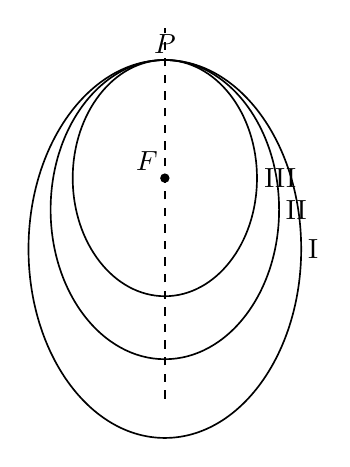
\begin{tikzpicture}[x=0.78cm, y=1.0cm, semithick, every node/.style={inner sep=1.3pt}]
  % 对称轴
  \draw[dashed] (0,-1.7) -- (0,3.0);

  % 椭圆 I：中心 (0,0.2)，半长轴 2.4、半短轴 2.22
  \draw (0,0.2) ellipse [x radius=2.22, y radius=2.4];
  % 椭圆 II：中心 (0,0.7)，半长轴 1.9、半短轴 1.86
  \draw (0,0.7) ellipse [x radius=1.86, y radius=1.9];
  % 圆 III：圆心 F(0,1.1)，半径 1.5
  \draw (0,1.1) circle [radius=1.5];

  % 焦点与切点
  \fill (0,1.1) circle (1.7pt);
  \node[above left=1pt] at (0,1.1) {$F$};
  \node[above] at (0,2.62) {$P$};

  \node[right] at (2.26,0.20) {I};
  \node[right] at (1.90,0.70) {II};
  \node[right] at (1.55,1.10) {III};
\end{tikzpicture}
\end{center}
\nopagebreak[4]
\end{question}
\gkpart{二、填空题}

\begin{question}
\gkti{11}设 $z_1$ 是复数，$z_2=z_1-\mathrm i\overline{z_1}$（其中 $\overline{z_1}$ 表示 $z_1$ 的共轭复数），已知 $z_2$ 的实部是 $-1$，则 $z_2$ 的虚部为\gkblank{}。

\end{question}
\begin{question}
\gkti{12}在 $\triangle ABC$ 中，三个角 $A$，$B$，$C$ 的对边边长分别为 $a=3$，$b=4$，$c=6$，则 $bc\cos A+ca\cos B+ab\cos C$ 的值为\gkblank{}。

\end{question}
\begin{question}
\gkti{13}已知函数 $f(x)=x^2+2x+a$，$f(bx)=9x^2-6x+2$，其中 $x\in\mathbf R$，$a$，$b$ 为常数，则方程 $f(ax+b)=0$ 的解集为\gkblank{}。

\end{question}
\begin{question}
\gkti{14}已知函数 $f(x)=2^x$，等差数列 $\{a_n\}$ 的公差为 $2$。若 $f(a_2+a_4+a_6+a_8+a_{10})=4$，则 $\log_2[f(a_1)\cdot f(a_2)\cdot f(a_3)\cdots f(a_{10})]=$\gkblank{}。

\end{question}
\begin{question}
\gkti{15}观察下列等式：

\nopagebreak[4]
\[\sum_{i=1}^ni=\frac12n^2+\frac12n,\]

\nopagebreak[4]
\[\sum_{i=1}^ni^2=\frac13n^3+\frac12n^2+\frac16n,\]

\nopagebreak[4]
\[\sum_{i=1}^ni^3=\frac14n^4+\frac12n^3+\frac14n^2,\]

\nopagebreak[4]
\[\sum_{i=1}^ni^4=\frac15n^5+\frac12n^4+\frac13n^3-\frac1{30}n^2,\]

\nopagebreak[4]
\[\sum_{i=1}^ni^5=\frac16n^6+\frac12n^5+\frac5{12}n^4-\frac1{12}n^2,\]

\nopagebreak[4]
\[\sum_{i=1}^ni^6=\frac17n^7+\frac12n^6+\frac12n^5-\frac16n^3+\frac1{42}n^2,\]

\nopagebreak[4]
\[\cdots\cdots\cdots\cdots\cdots\cdots\cdots\cdots\cdots\cdots\cdots\cdots\]

\nopagebreak[4]
\[\sum_{i=1}^ni^k=a_{k+1}n^{k+1}+a_kn^k+a_{k-1}n^{k-1}+a_{k-2}n^{k-2}+\cdots+a_1n+a_0,\]

可以推测，当 $k\geqslant2$（$k\in\mathbf N^*$）时，$a_{k+1}=\dfrac1{k+1}$，$a_k=\dfrac12$，$a_{k-1}=$\gkblank{}，$a_{k-2}=$\gkblank{}。

\end{question}
\gkpart{三、解答题}

\begin{question}
\gkti{16}已知函数 $f(t)=\sqrt{\dfrac{1-t}{1+t}}$，$g(x)=\cos x\cdot f(\sin x)+\sin x\cdot f(\cos x)$，$x\in\left(\pi,\dfrac{17\pi}{12}\right]$。

（1）将函数 $g(x)$ 化简成 $A\sin(\omega x+\varphi)+B$（$A>0$，$\omega>0$，$\varphi\in[0,2\pi)$）的形式；

（2）求函数 $g(x)$ 的值域。

\end{question}
\begin{question}
\gkti{17}袋中有 $20$ 个大小相同的球，其中记上 $0$ 号的有 $10$ 个，记上 $n$ 号的有 $n$ 个（$n=1,2,3,4$）。现从袋中任取一球。$\xi$ 表示所取球的标号。

（1）求 $\xi$ 的分布列，期望和方差；

（2）若 $\eta=a\xi+b$，$E\eta=1$，$D\eta=11$，试求 $a$，$b$ 的值。

\Needspace{0.4\textheight}
\end{question}
\begin{question}
\gkti{18}如图，在直三棱柱 $ABC-A_1B_1C_1$ 中，平面 $A_1BC\perp$ 侧面 $A_1ABB_1$。

（1）求证：$AB\perp BC$；

（2）若直线 $AC$ 与平面 $A_1BC$ 所成的角为 $\theta$，二面角 $A_1-BC-A$ 的大小为 $\varphi$，试判断 $\theta$ 与 $\varphi$ 的大小关系，并予以证明。
\nopagebreak[4]
\begin{center}% 2008 年湖北卷理科第 18 题：直三棱柱 ABC-A1B1C1，平面 A1BC ⊥ 侧面 A1ABB1。
% 来源 PDF：gaokaomath-src/普通高考/2008/2008湖北文.pdf
% SHA-256：54077e9ac5227f015a8972bfc4c4415b503b31acdf0a6e7cd51782afa098a112
% 原页：2008湖北理.pdf 第 2 页（A3 三栏）第 1 栏，书页码 450。
% 重绘依据：按原页斜投影：上底 A1（左上）、C1（右上）、B1（右中），下底 A（左下）、C（右下）、
%   B（下中）；可见棱 A1C1、A1B1、B1C1、AA1、BB1、CC1、AB、BC 与对角 A1B 实线，
%   A—C 为被遮挡的底边（虚线）。
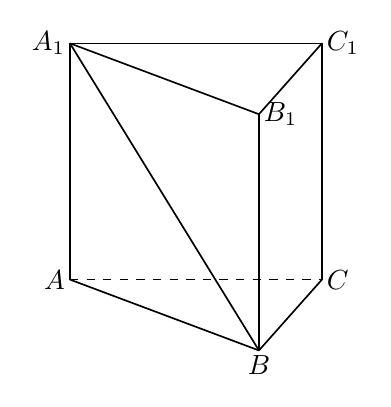
\begin{tikzpicture}[scale=1.0, semithick, every node/.style={inner sep=1.5pt}]
  \coordinate (A) at (0.20,0.40);
  \coordinate (C) at (3.40,0.40);
  \coordinate (B) at (2.60,-0.50);
  \coordinate (A1) at (0.20,3.40);
  \coordinate (C1) at (3.40,3.40);
  \coordinate (B1) at (2.60,2.50);

  \draw (A1) -- (C1);
  \draw (A1) -- (B1);
  \draw (B1) -- (C1);
  \draw (A) -- (A1);
  \draw (B) -- (B1);
  \draw (C) -- (C1);
  \draw (A) -- (B);
  \draw (B) -- (C);
  \draw (A1) -- (B);
  \draw[dashed] (A) -- (C);

  \node[left] at (A) {$A$};
  \node[below] at (B) {$B$};
  \node[right] at (C) {$C$};
  \node[left] at (A1) {$A_1$};
  \node[right] at (B1) {$B_1$};
  \node[right] at (C1) {$C_1$};
\end{tikzpicture}
\end{center}
\nopagebreak[4]
\Needspace{0.4\textheight}
\end{question}
\begin{question}
\gkti{19}如图，在以点 $O$ 为圆心，$|AB|=4$ 为直径的半圆 $ADB$ 中，$OD\perp AB$，$P$ 是半圆弧上一点，$\angle POB=30^\circ$，曲线 $C$ 是满足 $||MA|-|MB||$ 为定值的动点 $M$ 的轨迹，且曲线 $C$ 过点 $P$。

（1）建立适当的平面直角坐标系，求曲线 $C$ 的方程；

（2）设过点 $D$ 的直线 $l$ 与曲线 $C$ 相交于不同的两点 $E$、$F$。若 $\triangle OEF$ 的面积不小于 $2\sqrt2$，求直线 $l$ 斜率的取值范围。
\nopagebreak[4]
\begin{center}% 2008 年湖北卷理科第 19 题：以 O 为圆心、|AB|=4 为直径的半圆 ADB，OD ⊥ AB，P 在半圆弧上，
%   ∠POB=30°。
% 来源 PDF：gaokaomath-src/普通高考/2008/2008湖北理.pdf
% SHA-256：54077e9ac5227f015a8972bfc4c4415b503b31acdf0a6e7cd51782afa098a112
% 原页：2008湖北理.pdf 第 2 页（A3 三栏）第 1 栏，书页码 450。
% 绘制依据：按原页画上半圆（圆心 O、半径 2），AB 水平、D 在最高点，P 位于 B 一侧 30° 处并连 OP。
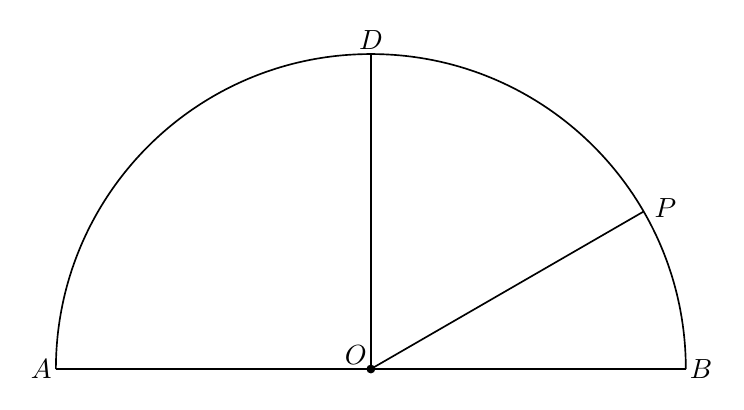
\begin{tikzpicture}[scale=2.0, semithick, every node/.style={inner sep=1.2pt}]
  % 半圆弧（上半）
  \draw (2,0) arc[start angle=0, end angle=180, radius=2];

  % 直径 AB 与半径 OD、OP
  \draw (-2,0) -- (2,0);
  \draw (0,0) -- (0,2);
  \draw (0,0) -- (30:2);

  \fill (0,0) circle (0.8pt);

  \node[left] at (-2,0) {$A$};
  \node[right] at (2,0) {$B$};
  \node[above] at (0,2) {$D$};
  \node[above left] at (0,0) {$O$};
  \node[right] at (30:2.05) {$P$};
\end{tikzpicture}
\end{center}
\nopagebreak[4]
\end{question}
\begin{question}
\gkti{20}水库的蓄水量随时间而变化。现用 $t$ 表示时间，以月为单位，年初为起点。根据历年数据，某水库的蓄水量（单位：亿立方米）关于 $t$ 的近似函数关系式为

\nopagebreak[4]
\[V(t)=\begin{cases}(-t^2+14t-40)\mathrm e^{\frac14t}+50,&0<t\leqslant10,\\ 4(t-10)(3t-41)+50,&10<t\leqslant12.\end{cases}\]

（1）该水库的蓄水量小于 $50$ 的时期称为枯水期。以 $i-1<t<i$ 表示第 $i$ 月份（$i=1,2,\cdots,12$），同一年内哪几个月份是枯水期？

（2）求一年内该水库的最大蓄水量（取 $\mathrm e=2.7$ 计算）。

\end{question}
\begin{question}
\gkti{21}已知数列 $\{a_n\}$ 和 $\{b_n\}$ 满足：$a_1=\lambda$，$a_{n+1}=\dfrac23a_n+n-4$，$b_n=(-1)^n(a_n-3n+21)$，其中 $\lambda$ 为实数，$n$ 为正整数。

（1）对任意实数 $\lambda$，证明数列 $\{a_n\}$ 不是等比数列；

（2）试判断数列 $\{b_n\}$ 是否为等比数列，并证明你的结论；

（3）设 $0<a<b$，$S_n$ 为数列 $\{b_n\}$ 的前 $n$ 项和。是否存在实数 $\lambda$，使得对任意正整数 $n$，都有 $a<S_n<b$？若存在，求 $\lambda$ 的取值范围；若不存在，说明理由。

\end{question}